\documentclass{article}
\usepackage{geometry, hyperref, minted,xcolor,setspace}
\usepackage{animate}
\geometry{margin=1in}
\usepackage{graphicx} % Required for inserting images

\title{RIFT Tutorial \\
\large 05: Generating Runs on Synthetic Data}
\author{Katelyn J. Wagner}
\date{}

\begin{document}
\setstretch{1.25}
\maketitle

Injection and recovery testing is a critical tool for validating and stress-testing our pipeline. We can assess how accurately and precisely the pipeline recovers source parameters under controlled conditions by injecting a known GW signal into simulated or low-noise background data and attempting to recover it. This process allows us to test the pipeline's robustness across a wide range of source properties (e.g., mass, spin, eccentricity), sampling configurations, and integration methods. It also helps us quantify things like the impact of waveform systematics (differences between the injected signal model and the model used for recovery) which can bias results if not properly accounted for. Basically, this type of test provides a ground truth framework for identifying biases, understanding uncertainties, and ensuring the pipeline is functioning as expected before applying it to real detector data.

\section*{Injection \& Recovery}
As usual, begin by sourcing your environment and/or setup script. The most common pitfall for new users is improperly set environment variables and paths. There are ways to automate sourcing these (i.e. modifying your \texttt{.bashrc}) but proceed carefully.

We will now create fake gravitational wave data and perform a test RIFT run. This is the procedure we use for systematics studies. The first step is to create the synthetic data.
\begin{figure}[h!]
    \centering
    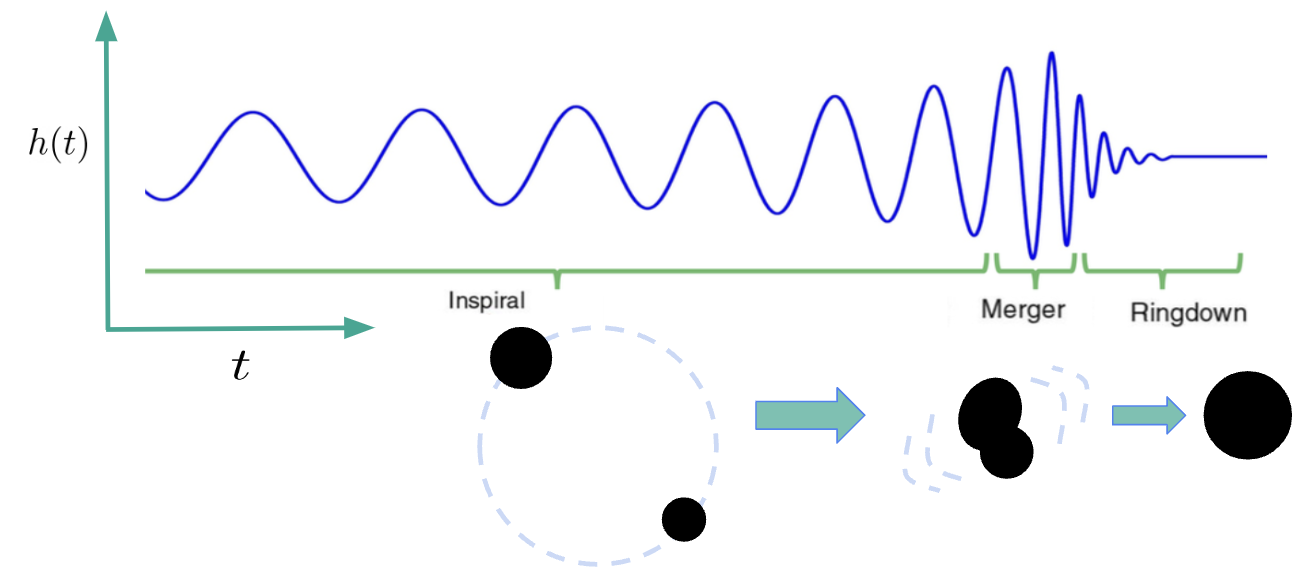
\includegraphics[width=0.75\linewidth]{data.png}
    \caption{A sample gravitational wave signal showing the merger stages.}
    \label{fig:data}
\end{figure}
To do this, we will combine a fake gravitational wave signal (created using a specified waveform model) with noise frames based on LIGO detector design. As expected, our data = signal + noise. The infrastructure to perform this already exists within the RIFT repository. It's best to checkout a new copy of the repo to perform these tests in. Note that this \textbf{will not be} the source where your conda environment access scripts. Be careful! From your home directory:

\begin{minted}[frame=single,obeytabs=true,tabsize=4,linenos,numbersep=-10pt]{bash}
    git clone https://github.com/oshaughn/research-projects-RIT.git
\end{minted}

Navigate to the \texttt{pp} directory:
\begin{minted}[frame=single,obeytabs=true,tabsize=4,linenos,numbersep=-10pt]{bash}
    cd research-projects-RIT/MonteCarloMarginalizeCode/Code/test/pp
\end{minted}

Add this directory to your path so that the scripts can find other supporting scripts within this directory.
\begin{minted}[frame=single,obeytabs=true,tabsize=4,linenos,numbersep=-10pt]{bash}
    export PATH=${PATH}:`pwd`
\end{minted}
The relevant scripts are \texttt{pp\_RIFT} and \texttt{pp\_RIFT\_with\_ini}. New users should use \texttt{pp\_RIFT\_with\_ini} unless they have a reason not to, as it directly uses the setup procedures we also use for production level runs on real data. You will modify \texttt{sample\_pp\_w\_ini.ini} (the copy that comes in \texttt{rift\_O4c} should be fine), but you will need to copy PSDs from the author's home directory for now:
\begin{minted}[frame=single,obeytabs=true,tabsize=4,linenos,numbersep=-10pt]{bash}
    cp /home/katelyn.wagner/*psd.xml.gz .
\end{minted}
Open the ini file and change the \texttt{username} to match yours in the \texttt{[make\_workflow]} section of the ini file. All other settings are fine for a test run, but note that these are the values a user modifies to create custom systematics runs. You are ready to build the workflow. From this directory, run:
\begin{minted}[frame=single,obeytabs=true,tabsize=4,linenos,numbersep=-10pt]{bash}
    pp_RIFT_with_ini --use-ini sample_pp_w_ini.ini
\end{minted}
This creates a new directory (named by “working\_directory” as specified in the ini file) which contains
\begin{itemize}
    \item An injection file containing the source parameters: \texttt{mdc.xml.gz}
    \item A directory containing the signal frames: \texttt{signal\_frames}
    \item A directory containing signal+noise frames: \texttt{combined\_frames}
    \item The event directory: \texttt{analysis\_event\_0/}
    \item A dag that contains info for condor to submit the job: \texttt{master.dag}
\end{itemize}
Navigate into the event directory and test a single ILE instance to make sure the setup worked:
\begin{minted}[frame=single,obeytabs=true,tabsize=4,linenos,numbersep=-10pt]{bash}
    cd test_pp/analysis_event_0/rundir
    ./command-single.sh
\end{minted}
\newpage
There will be a bunch of output, but once you see output like the following, you know the job will run on the cluster:
\begin{figure}[h!]
    \centering
    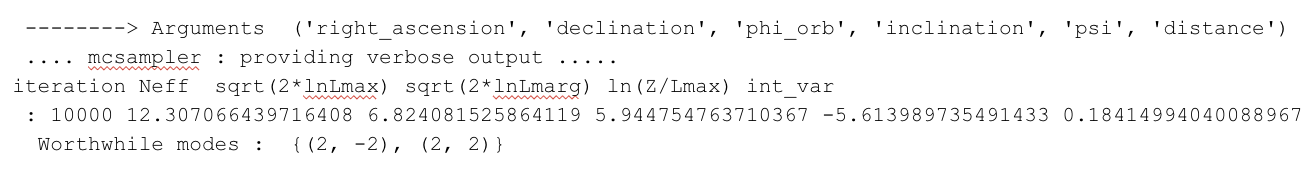
\includegraphics[width=0.9\linewidth]{output.png}
    \label{fig:output}
\end{figure}
There might be some errors about \texttt{lalym}, but you can ignore them.
Finally, you can submit the job to the cluster using HTCondor and watch the progress:
\begin{minted}[frame=single,obeytabs=true,tabsize=4,linenos,numbersep=-10pt]{bash}
    condor_submit_dag -import_env master.dag
    watch condor_q
\end{minted}

You always want jobs in the RUN and IDLE columns, otherwise something is wrong:
\begin{figure}[h!]
    \centering
    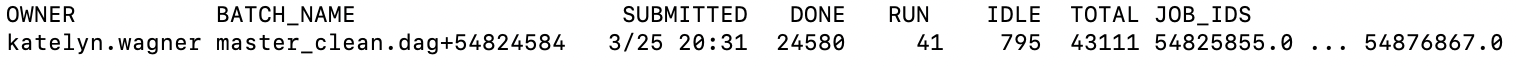
\includegraphics[width=0.9\linewidth]{condor.png}
    \label{fig:condor}
\end{figure}
Congratulations! You just created synthetic signals, joined them with noise to create synthetic LIGO data, setup a RIFT run directory, and submitted your run to cluster computing resources.

For more extensive testing, users typically run this type of analysis on 100 events, and change the waveforms used in the ini file. Some common pitfalls:


\begin{itemize}
    \item \texttt{pp\_RIFT\_with\_ini} only checks if the \texttt{signal\_frames} and \texttt{combined\_frames} directories \textit{exist}, but not whether they were properly generated. Many users try to submit runs without these directories properly built. This can happen for a number of reasons, including but not limited to:
    \begin{itemize}
        \item SSH connection timing out (e.g., getting logged out of the cluster during a build). Try using \texttt{screen}.
        \item Failing to run \texttt{export PATH=\$\{PATH\}:\`pwd\`} each time you log in to build a rundir, which can cause \texttt{add\_frames.py} to be unavailable to \texttt{pp\_RIFT\_with\_ini}.
    \end{itemize}
    \item Forgetting to source \texttt{setup.sh}, so things like the singularity image and the accounting group/user are not properly set in the sub files.
\end{itemize}

If you made a rundir but realized your settings were not correct, you can keep the \texttt{mdc.xml.gz} file, the \texttt{signal\_frames} directory, and \texttt{combined\_frames} directory. Delete the \texttt{analysis\_event\_XX} directories, the \texttt{pseduo\_ini.ini}, and the \texttt{master.dag}. Then, rerun \texttt{pp\_RIFT\_with\_ini} using the same ini file. It will detect the existence of the frames and just rebuild the analysis directories. If you'd like to keep the original analysis directories but perform a rerun, simply \texttt{cp -r} the \texttt{mdc.xml.gz} file, the \texttt{signal\_frames} directory, and \texttt{combined\_frames} directory to your new location, change the dir name in your ini file, and rerun \texttt{pp\_RIFT\_with\_ini} as usual.

\noindent - If you're using the OSG, when you run \texttt{pp\_RIFT\_with\_ini}, add the \texttt{--use-osg} flag.

\noindent - If you're using an SEOB model, when you run \texttt{pp\_RIFT\_with\_ini}, add the \texttt{--use-gwsignal} flag to access the external waveform interface that is required for this waveform.

\noindent - For more settings information, visit the \href{https://rift-documentation.readthedocs.io/en/latest/index.html}{documentation}.

\end{document}
